%%
%% ****** ljmsamp.tex 13.06.2018 ******
%%
\documentclass[
11pt,%
tightenlines,%
twoside,%
onecolumn,%
nofloats,%
nobibnotes,%
nofootinbib,%
superscriptaddress,%
noshowpacs,%
centertags]%
{revtex4}
\usepackage{ljm}
\usepackage{listings}

\lstset{
language=C++,
basewidth=0.5em,
xleftmargin=45pt,
xrightmargin=45pt,
basicstyle=\small\ttfamily,
keywordstyle=\bfseries\underbar,
numbers=left,
numberstyle=\tiny,
stepnumber=1,
numbersep=10pt,
showspaces=false,
showstringspaces=false,
showtabs=false,
frame=trBL,
tabsize=2,
captionpos=t,
breaklines=true,
breakatwhitespace=false,
escapeinside={\%*}{*)}
}

\begin{document}

\titlerunning{RANS/ILES method optimization} % for running heads
\authorrunning{G.~I.~Savin, L.~A.~Benderskiy, D.~A.~Lyubimov, A.~A.~Rybakov} % for running heads

\title{RANS/ILES Method Optimization for Effective Calculations on Supercomuter}
% Splitting into lines is performed by the command \\
% The title is written in accordance with the rules of capitalization.

\author{\firstname{G.~I.}~\surname{Savin}}
\email[E-mail: ]{savin@jscc.ru} \affiliation{Joint
Supercomputer Center of the Russian Academy of Sciences (JSCC RAS)
--  Branch of Scientific Research Institute of System Analysis of
the Russian Academy of Sciences, Leninsky prospect 32a, Moscow,
119334, Russia}

\author{\firstname{L.~A.}~\surname{Benderskiy}}
\email[E-mail: ]{leosun.ben@gmail.com} \affiliation{Joint
Supercomputer Center of the Russian Academy of Sciences (JSCC RAS)
--  Branch of Scientific Research Institute of System Analysis of
the Russian Academy of Sciences, Leninsky prospect 32a, Moscow,
119334, Russia}

\author{\firstname{D.~A.}~\surname{Lyubimov}}
\email[E-mail: ]{dalyubimov@ya.ru} \affiliation{Joint Supercomputer
Center of the Russian Academy of Sciences (JSCC RAS) --  Branch of
Scientific Research Institute of System Analysis of the Russian
Academy of Sciences, Leninsky prospect 32a, Moscow, 119334, Russia}

\author{\firstname{A.~A.}~\surname{Rybakov}}
\email[E-mail: ]{rybakov.aax@gmail.com} \affiliation{Joint
Supercomputer Center of the Russian Academy of Sciences (JSCC RAS)
-- Branch of Scientific Research Institute of System Analysis of the
Russian Academy of Sciences, Leninsky prospect 32a, Moscow, 119334,
Russia}


\firstcollaboration{(Submitted by A.~M.~Elizarov)} % Add if you know submitter.
%\lastcollaboration{ }

\received{June 13, 2018} % The date of receipt to the editor, i.e. December 06, 2017

\begin{abstract}
The article discusses the use of the RANS/ILES method for  modeling
gas-dynamic processes in a combustion chamber, described using an
axisymmetric block-structured computational grid. For these
calculations, the approaches of the linked border conditions and the
fragmentation of the computational grid are used, which allows to
effectively calculate this problem on a supercomputer, achieving
acceleration by more than two orders of magnitude, using a total of
32 computing nodes.
\end{abstract}

\subclass{76Nxx, 76Fxx, 68N19} % Enter 2010 Mathematics Subject Classification.

\keywords{computation fluid dynamics, RANS/ILES, calculation grid,
grid crushing, linked border conditions.} % Include keywords separeted by comma.

\maketitle

% Text of article starts here.

\section{Introduction}

The complex geometry of the combustion chamber and the different scale of the
flame tube and fuel supply devices requires the use of computational grid with
 a very large number of cells for adequately describe all the features of the flow,
  even when using high-resolution methods.
On the other hand, the geometry of the front device has a structure that is periodic in the azimuthal direction.
This formally allows us to calculate only the sector of the flame
tube with the conditions of periodicity on its lateral sides.
However, it is known that separated flows in annular diffusers can have azimuthal inhomogeneity with axisymmetric distribution of flow parameters at the inlet \cite{Lyub_Diffusers}.
This effect can only be detected when calculating the entire flame tube but not its sector.

Numeric simulation of combustion chamber sector require to solve a number
 of tasks on scaling the calculations. It is necessary to take into account the
 condition of periodicity in grid decomposition. This article is aimed at describing
 the mechanisms of grid decomposition with such boundary conditions and testing the decomposition method.

\section{Numerical method}

The RANS/ILES (Reynolds Averaged Navier--Stokes -- RANS, Implicit
Large Eddy Simulation -- ILES) method is based on Navier--Stokes
equations describing the flow of a compressible gas. The transport
equation for turbulence model is written in conservative form for
curvilinear coordinate system. The grid lines coincide with the
boundaries of computational domain, the nozzle surface. Hybrid
RANS/ILES method \cite{i1,Ben_Lyub_Chest_RANS_ILES} is used to solve
equations. The RANS method is used near walls and ILES is used in
the rest of the computational domain. Scheme viscosity plays a role
of a subgrid scale (SGS) model. The Roe method was applied to
calculate non-viscous flux on cell faces. The high resolution of
this method is provided by using a monotone difference scheme MP9
\cite{i2} with upwind 9th-order approximation to calculate flow
parameters on cell faces. This approach has been successfully used
in \cite{i3}. Diffusion fluxes are calculated on cell faces with
second-order approximation by central differences. The time
discretization is made with second order by implicit scheme and with
integration by double time method. The Spalart--Allmaras turbulence
model is used in RANS region. The WENO-5 scheme \cite{i2} is used to
calculate convective flows on cell faces in the difference analog of
turbulence model equation. In LES region, the Spalart--Allmaras
turbulence model is modified so that the turbulent viscosity is
equated to zero.
This is achieved by changing the distance in dissipative term of
 turbulence model equation. The modified distance $\tilde{d}$ is calculated by the formula %(\ref{eqn:d}).
\begin{equation}
\label{eqn:d}
\tilde{d} =
\begin{cases}
d, d \le C_{ILES}\Delta_{MAX},\\
0, d > C_{ILES}\Delta_{MAX},
\end{cases}
\end{equation}
where $d$ is the distance from the wall to the cell center,
$\Delta_{MAX}$ is the maximum size of the cell, $C_{ILES}$ is
constant defining position of transition from RANS to ILES and equal
0,65.

\section{Computational grids and simulation parameters}

The computational grid of the full-size flame tube is obtained by
cloning and rotating the grid of the flame tube sector. The size of
the grid for the sector is $9,4 \times 10^6$ cells, for a full-size
flame tube there is $94 \times 10^6$ cells. The supply of passive
impurity, simulating fuel, is made through the holes on the
stabilizer, as well as through the holes on the ends of the pylons
located above and below the stabilizer. The general view of the
front device, as well as a grid on its surface, are shown in
Fig.~\ref{fig:p1}, Fig.~\ref{fig:p2} and Fig.~\ref{fig:p3}.

\begin{figure}[ht]
\setcaptionmargin{5mm}
\onelinecaptionstrue
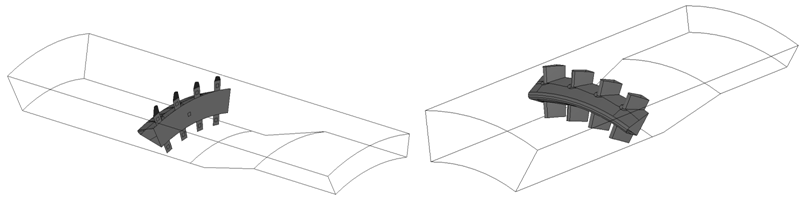
\includegraphics[width=0.7\textwidth]{pics/p1.png}
\captionstyle{normal}\caption{The general view of the computational model for sector of flame tube.}
\label{fig:p1}
\end{figure}

\begin{figure}[ht]
\setcaptionmargin{5mm}
\onelinecaptionstrue
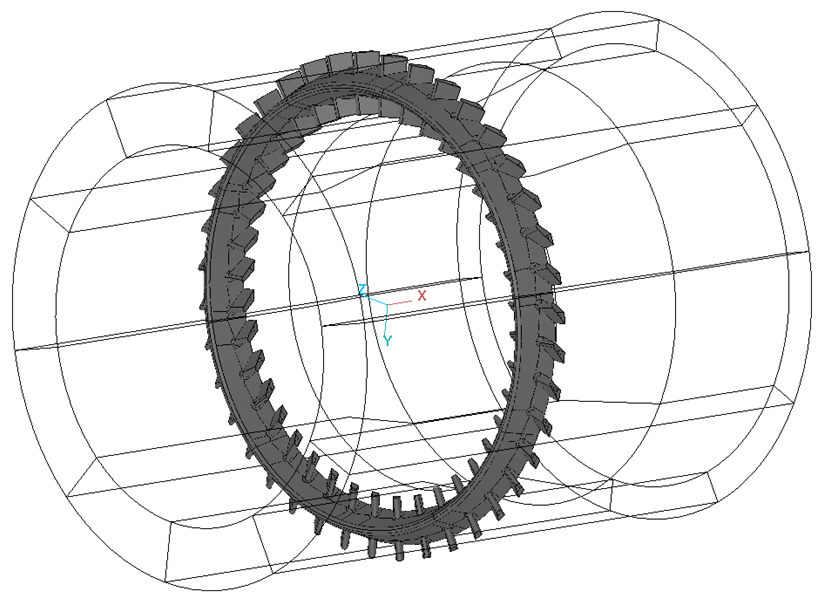
\includegraphics[width=0.55\textwidth]{pics/p2.png}
\captionstyle{normal}\caption{General view of the computational
model for full geometry of flame tube.} \label{fig:p2}
\end{figure}

\begin{figure}[ht]
\setcaptionmargin{5mm}
\onelinecaptionstrue
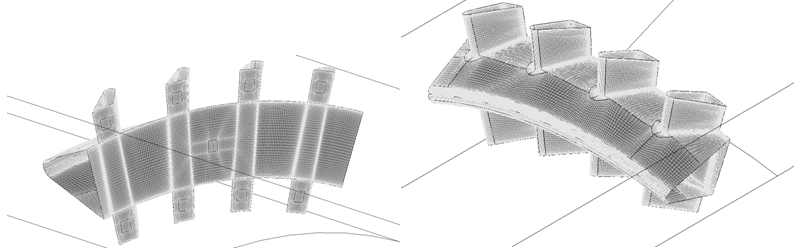
\includegraphics[width=0.6\textwidth]{pics/p3.png}
\captionstyle{normal}\caption{The computational grid on front device and pylons.}
\label{fig:p3}
\end{figure}

Total temperature and pressure is 300 K and $10^5$ Pa at the inlet
of the flame tube. The twist angle of flow is $40^{\circ}$. Static
pressure at the end of flame tube is 89560 Pa. The velocity of flow
between pylons compose 100--120 m/s the inlet velocity is 32 m/s for
this pressure ratio. The velocity vector and the total temperature
is fixed at the hole on pylons end. Velocity of passive impurity on
pylons end is 32 m/s and twist angle is $40^{\circ}$. Velocity of
passive impurity on front device is 42 m/s and angle is a normal to
the end of front device. The total temperature of passive impurity
is 300 K.

In Fig.~\ref{fig:p4} shows the fields of instantaneous distribution
of  axial velocity in sections passing through the holes on the hole
on the stabilizer. The essentially unsteady nature of the flow is
seen. The zone with a reverse flow is formed behind the stabilizer.
The flow is accelerated above and below the stabilizer due to
section load. The same can be seen in the Fig.~\ref{fig:p5} where
the isosurfaces of the concentration of a passive impurity are
shown. Due to the recirculation zone formation the jet of passive
impurity from the holes on the stabilizer propagates almost along
the surface of the front device.

\begin{figure}[ht]
\setcaptionmargin{5mm}
\onelinecaptionstrue
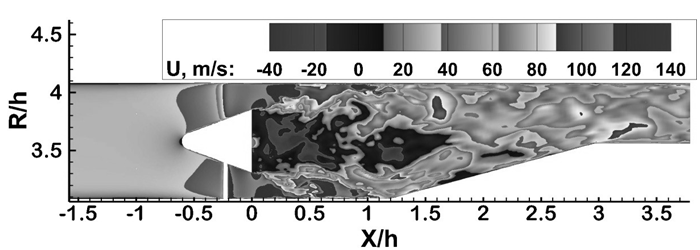
\includegraphics[width=0.5\textwidth]{pics/p4.png}
\captionstyle{normal}\caption{Instantaneous axial velocity
at longitudinal cut of flame tube ($h$ is inlet height of flame tube).}
\label{fig:p4}
\end{figure}

\begin{figure}[ht]
\setcaptionmargin{5mm}
\onelinecaptionstrue
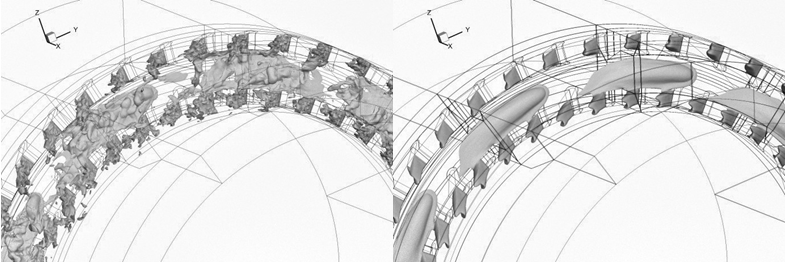
\includegraphics[width=0.75\textwidth]{pics/p5.png}
\captionstyle{normal}\caption{Instantaneous isosurface
 and time average isosurface of passive impurity for concentration 0,1.}
\label{fig:p5}
\end{figure}

The calculation results show a slight difference in the numerical
simulation of the flame tube for sector of $36^{\circ}$ and full
$360^{\circ}$. The recovery coefficient of the total pressure in the
outlet of flame tube is 6\% and 6,13\%. The difference in the
averaged flow parameters in the outlet is small and amounts to less
than 1\% for the distribution of the total and static pressure and
about 13\% for the distribution of the concentration of a passive
impurity. The greatest differences are observed in the distribution
of the pulsating characteristics of the flow, so the pressure
pulsations differ by 5--17\%, the energy of turbulence by 5--12\%.
In this case, the level of pulsations is about 0,2\% and 14--15\% of
the values of the averaged pressure and velocity in this section.
The rate of increase in the mixing completeness whole combustion
chamber is slightly lower (Fig.~6), however, the $\eta$ level at the
exit of the flame tube is almost the same for both cases. The mixing
completeness is determined by the ratio $\eta = \frac{1 -
C_{\max}}{1 - C_{av}}$, where $C_{\max}$ is maximum concentration in
the section and $C_{av}$ is averaging in cross-section value of
passive impurity concentration.

\begin{figure}[ht]
\setcaptionmargin{5mm}
\onelinecaptionstrue
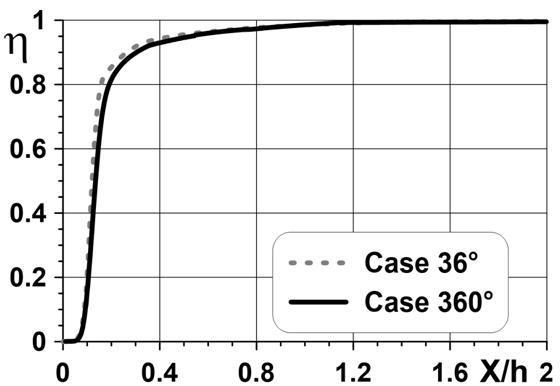
\includegraphics[width=0.35\textwidth]{pics/p6.png}
\captionstyle{normal}\caption{Distribution of the  completeness of
mixing along the length of the combustion chamber.} \label{fig:p6}
\end{figure}

The calculation results show a slight difference in the  numerical
simulation of the flame tube for sector of $36^{\circ}$ and full
$360^{\circ}$.

\section{Realization of linked border conditions}

The RANS/ILES method works with block-structured grids
\cite{Farrashkhalvat,Liseikin},  which consist of separate blocks
interconnected by interfaces. Each block of the computational grid
is an ordered three-dimensional array of cells, which can be
accessed by indices. This greatly simplifies the work with the grid
within one block. With each cell a set of gas-dynamic parameters is
associated. Each block of the computational grid has its own
three-dimensional curvilinear coordinate system, the axes of which
are directed along the edges of the block. Interfaces describing the
contact of blocks with each other contain information about the
coordinates of the touch of blocks areas (in terms of nodes of the
computational grid), as well as information about the matching of
coordinate systems of the related blocks. Some faces of the grid
blocks do not touch other blocks, but are the borders of the
computational domain. In this case, it is necessary to describe the
border conditions. This is done with the help of special objects
that describe the border conditions on a given rectangular section
of the block boundary \cite{Rybakov}.

When carrying out calculations, calculation grids consisting of
identical sectors are often used. That is, in essence, a grid with a
smaller number of cells, duplicated several times and rotated
relative to the original one around a given straight line. To obtain
a solution to the gas-dynamic problem, it is sufficient to perform
calculations for only one such sector. However, during the
calculations it is necessary to observe additional conditions. When
calculating a separate sector, it is necessary to take into account
that the output flows at the individual block borders must coincide
with the input flows at the borders of other blocks, and these
borders are spaced apart. Such border conditions will be called
linked. To increase the efficiency of the calculations using the
RANS/ILES method, this type of border conditions was implemented.

One of the main operations performed on the linked border conditions
is to determine whether they correspond to each other. With
automatic marking of the linked border conditions of the selected
sector of the computational grid, a compliance check is performed,
with which pairs of the linked border conditions are formed. Two
types of search for connections between border conditions are
implemented: border conditions combined by parallel transfer and
rotation around a given axis. To determine whether the two border
conditions are consistent with each other, it is needed to combine
them with the help of a given type of movement so that their centers
coincide, and then check whether their corner nodes coincide
(Fig.~\ref{fig:match3}).

\begin{figure}[ht]
\setcaptionmargin{5mm}
\onelinecaptionsfalse
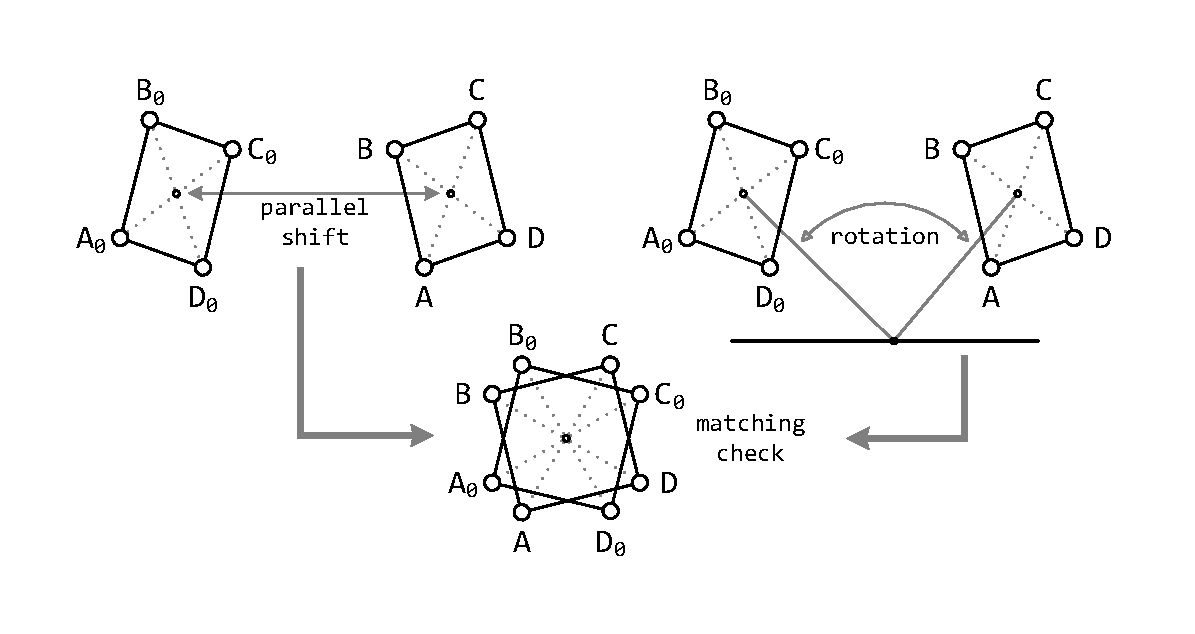
\includegraphics[width=0.85\textwidth]{pics/match3.pdf}
\captionstyle{normal} \caption{Connection of linked border
conditions to each other  using parallel shift and rotation around a
straight line.} \label{fig:match3}
\end{figure}

Checking the coincidence of the corner nodes of two potentially
linked border conditions is determined by considering four possible
cases, taking into account the renaming of vertices: the quadrangle
$A_0B_0C_0D_0$ can coincide with one of the quadrangles $ABCD$,
$DABC$, $CDAB$, $BCDA$ (Fig.~\ref{fig:match}).

\begin{figure}[h]
\setcaptionmargin{5mm}
\onelinecaptionstrue
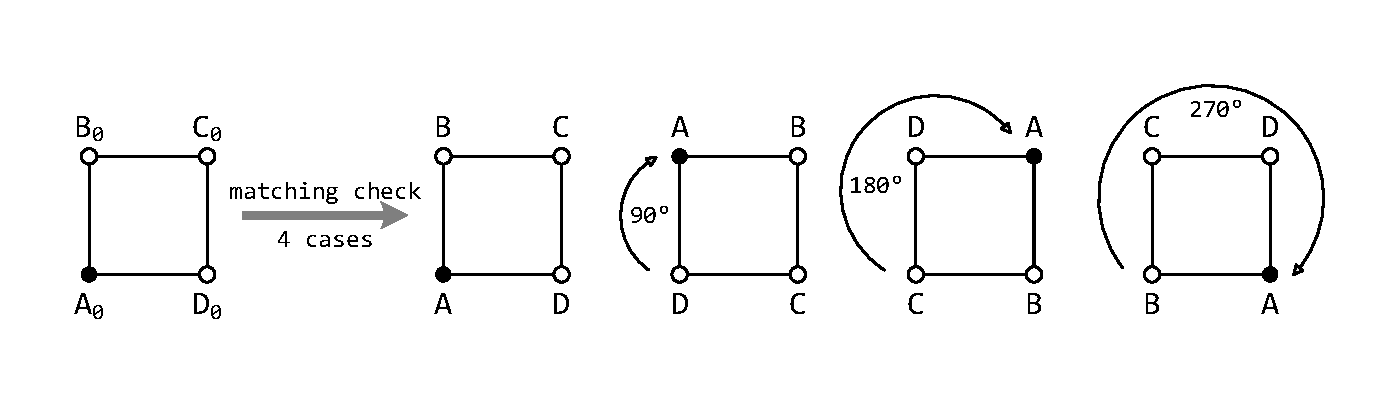
\includegraphics[width=0.95\textwidth]{pics/match.pdf}
\captionstyle{normal}\caption{Four cases for checking the
coincidence of the corner points of the border conditions.}
\label{fig:match}
\end{figure}

The order of checking the correspondence of the corner  nodes
$A_0B_0C_0D_0$ and $ABCD$ of the two border conditions is presented
in Fig.~\ref{fig:match2}. In addition to the fact that the corner
nodes of a pair of border conditions coincide, a correspondence
between their coordinate systems is also established. This allows
for any cell of a single border condition to find the corresponding
cell from the associated border condition. All further
transformations of the associated border conditions (renaming,
splitting the border condition or parent blocks) are performed only
simultaneously.

\begin{figure}[h]
\setcaptionmargin{5mm}
\onelinecaptionstrue
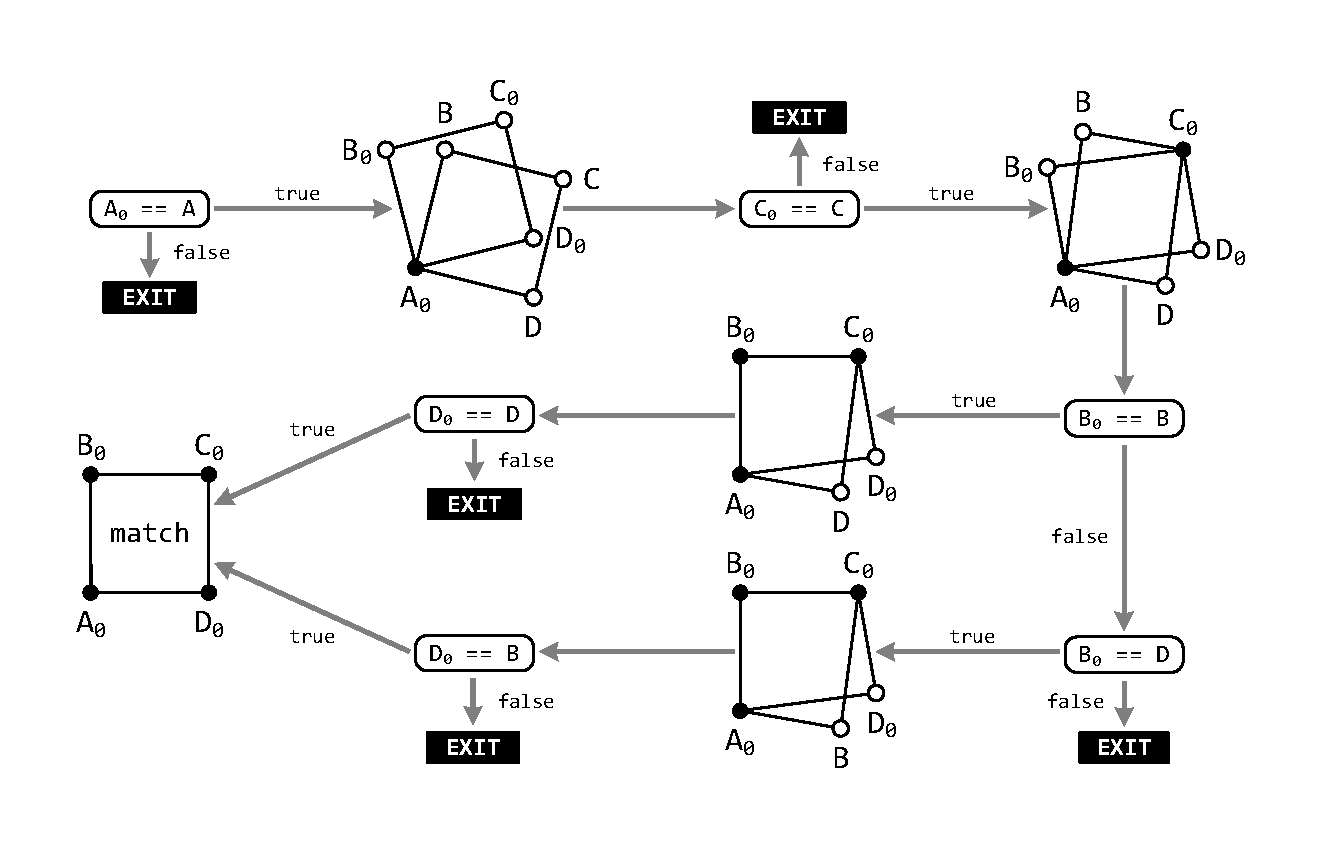
\includegraphics[width=0.9\textwidth]{pics/match2.pdf}
\captionstyle{normal}\caption{Checking the coincidence  of the
corner points of the border conditions.} \label{fig:match2}
\end{figure}

\section{Scalability of calculations investigation  when cutting the computational grid}

In this section, we describe the experimental launches and analyze
the scalability results obtained using the mechanisms of coupled
border conditions and fragmentation of the computational grid.

For testing, we used a computational grid describing the flame tube
and containing 94 million cells (we will call it a complete grid).
The mechanism of linked border conditions allowed us to replace the
calculations on this complete grid with calculations made on a
sector representing the $1/10$ part of the original grid (36 degrees
relative to the $OX$ axis). The computational grid describing one
sector contains 10,7 million cells, which is 9 times smaller than
the initial grid. At the same time, the calculation time is also
reduced by 9 times.

The experiments were performed on a segment of the MVS-10P
supercomputer  located at the JSCC RAS. This segment consists of
computing nodes based on Intel Xeon Phi Knights Landing 7290
microprocessors \cite{Jeffers_KNL}. From 1 to 32 computing nodes
were used for launches.

First, calculations were carried out on a complete grid. This grid
contains 300 calculation blocks, calculations on it are scaled  to
32 nodes linearly with MPI \cite{Queen} (the execution time of
calculations at 32 nodes is less than the calculation time on one
node by almost 32 times).

The computational grid describing one sector contains only 30 nodes,
so  the calculations on it are much worse scaled. To analyze the
scalability, crushing of this grid was performed by dividing the
largest block in half. In this algorithm, at each iteration, a block
is selected that contains the largest number of cells and is divided
in half. The algorithm finishes its work when the resulting blocks
can be distributed between the specified number of processes in such
a way that the maximum deviation from the average value does not
exceed the specified threshold. The Table~\ref{tab:grids} shows
examples of crushing, for which calculations were subsequently made.

\begin{table}[!ht]
\setcaptionmargin{0mm}
\onelinecaptionsfalse
\captionstyle{flushleft}
\caption{Characteristics of computational grids.}
\bigskip
\begin{tabular}{|c|c|c|c|c|}
\hline
grid description & blocks/scopes & interfaces & border conditions & linked border cond. \\
\hline
360 deg. (94 mln cells) & 300 & 1 796 & 1 643 & 0 \\
36 deg. (10,7 mln cells) & 30 & 152 & 204 & 14 \\
\hline
36 deg., cut for 16 proc. (10\% dev.) & 39 & 224 & 218 & 14 \\
36 deg., cut for 32 proc. (10\% dev.) & 54 & 340 & 248 & 14 \\
36 deg., cut for 64 proc. (10\% dev.) & 170 & 982 & 429 & 23 \\
\hline
36 deg., cut for 64 proc. (1\% dev.) & 383 & 2 356 & 682 & 34 \\
\hline
\end{tabular}
\label{tab:grids}
\end{table}

In Fig.~\ref{fig:g_36_2} adjacency graphs of computational grids
blocks obtained as a result of crushing are presented. The nodes of
the adjacency graph of the computational grid blocks are the centers
of the grid blocks. Two nodes of the graph are connected by an edge
if the two corresponding blocks are adjacent.

\begin{figure}[ht]
\setcaptionmargin{5mm}
\onelinecaptionsfalse
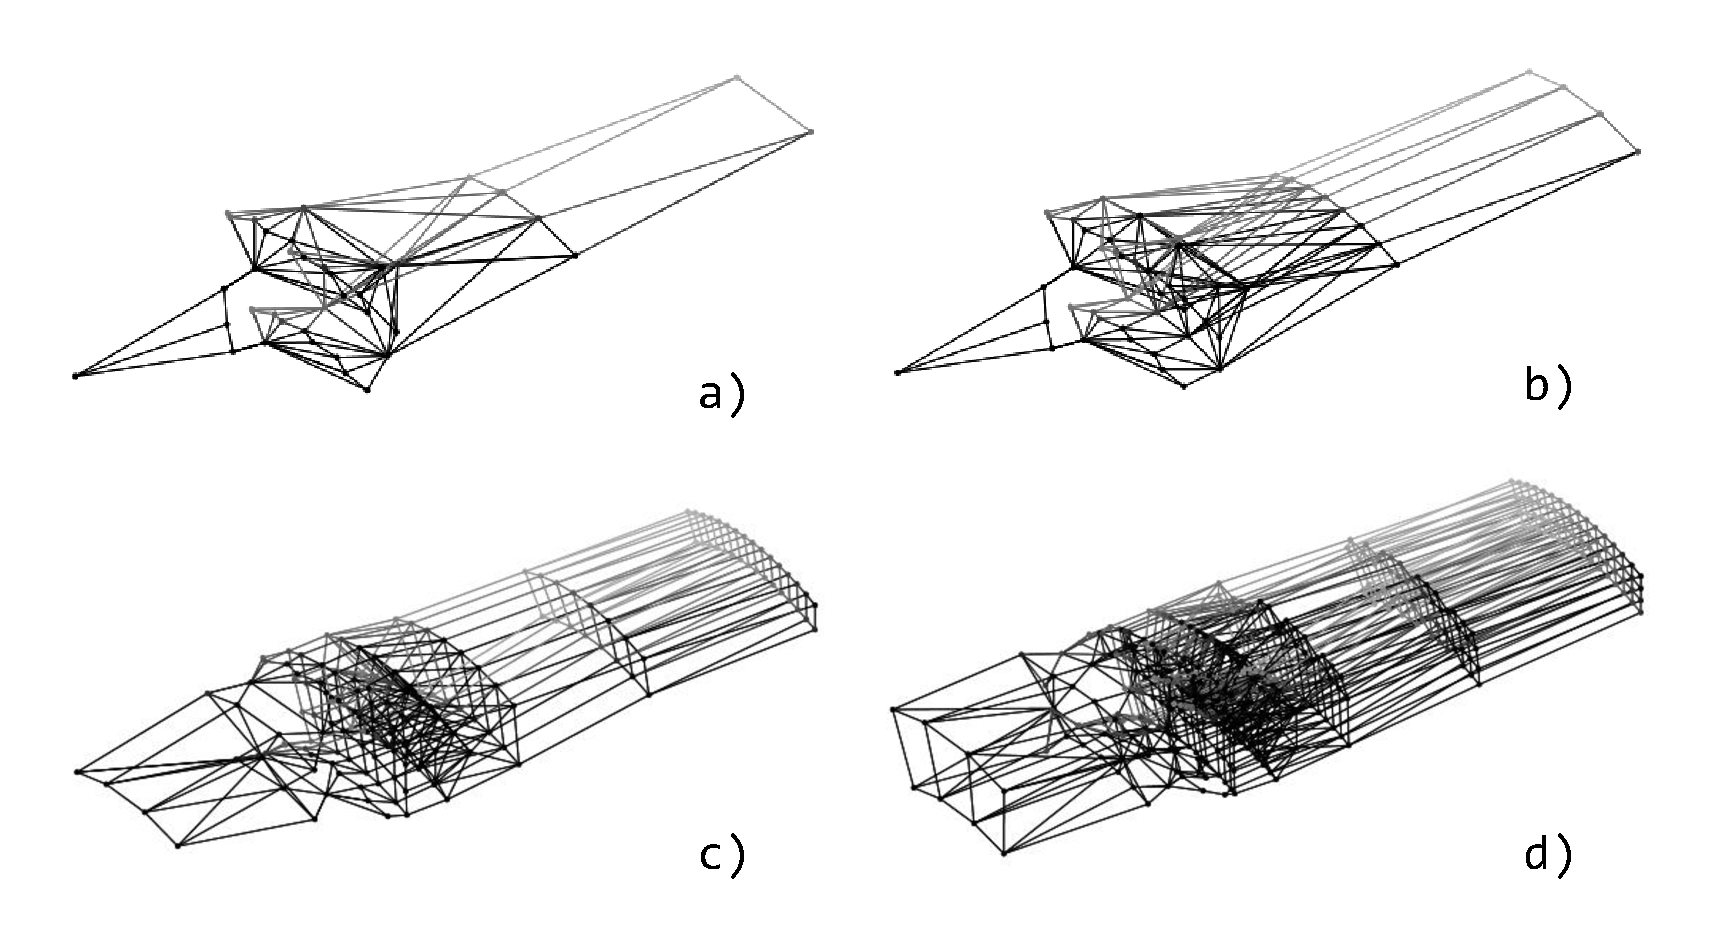
\includegraphics[width=0.9\textwidth]{pics/g_36_2.pdf}
\captionstyle{normal}\caption{Borders adjacency graphs for different
cases of computational grid cutting:  a -- cutting for 16 processes
(10\% deviation), b -- cutting for 32 processes (10\% deviation), c
-- cutting for 64 processes (10\% deviaton), d -- cutting for 64
processes (1\% deviation).} \label{fig:g_36_2}
\end{figure}

Fig.~\ref{fig:plot_36_scaling_2} shows the data of calculation runs
performed on the same sector (small grid) with various parameters of
the grid crushing. It can be seen that the acceleration of
calculations on the initial grid reaches approximately 4--5, and
then regardless of the number of nodes used do not change. This
indicates that there is a large block in the grid, so the processing
speed of the entire grid is limited from below by the processing
speed of this block by one process. When cutting the grid for
distribution by 16 processes (with a maximum deviation of 10\%), the
scaling of the calculations improves, but with an increase in the
number of computing nodes to 16 or more, the same effect is
observed. When cutting the grid for distribution to 32 or 64
processes (with a maximum deviation of 10\%), the results of scaling
are much better. The dependence of the acceleration on the number of
nodes used becomes almost linear, although with a large number of
computational nodes, some fluctuations are observed.

\begin{figure}[ht]
\setcaptionmargin{5mm}
\onelinecaptionstrue
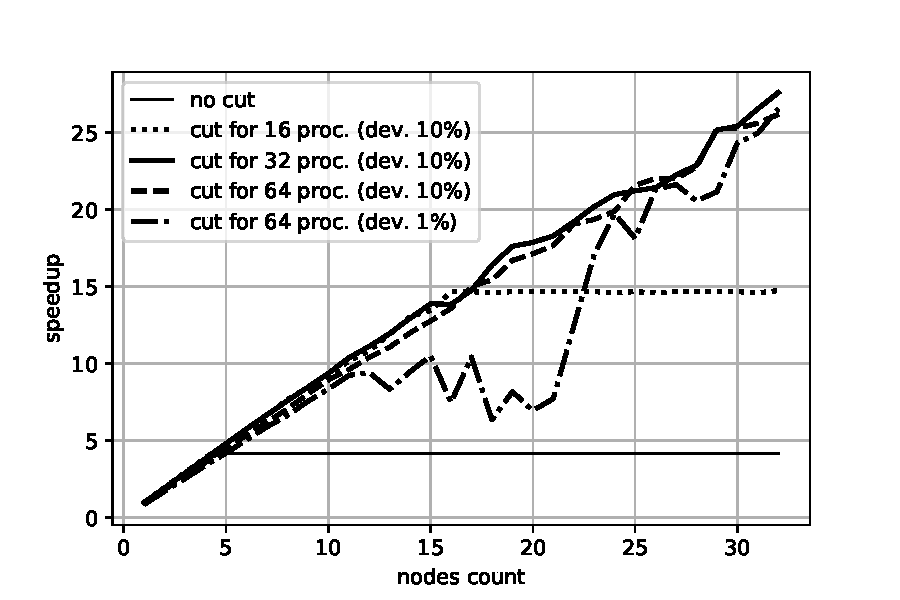
\includegraphics[width=0.7\textwidth]{pics/plot_36_scaling_2.pdf}
\captionstyle{normal}\caption{Graph scaling calculations when  using
different options for cutting the grid.}
\label{fig:plot_36_scaling_2}
\end{figure}

Also in Fig.~\ref{fig:plot_36_scaling_2} the data of the  launches
performed on the grid, which is fragmented very finely. The grid was
cutted for distribution to 64 processes, while the maximum allowable
deviation from the average computational load was taken as 1\%. The
graph shows a very serious drawdown of scaling in the range from 10
to 20 computing nodes. This is due to the fact that unnecessarily
fine crushing leads to the appearance of a huge number of
computational blocks and interfaces between them. In some cases,
blocks can be distributed between processes so that the amount of
data involved in interprocess exchanges between them, becomes
critical. In such situations it is necessary to take into account
the factor of interprocess exchanges or not to resort to excessive
fragmentation of the grid.

\section{Conclusion}

The results of practical experiments have shown that the  mechanisms
for preparing the block-structured computational grid for the
RANS/ILES method help to achieve multiple acceleration of
calculations when performing calculations on a supercomputer. In
particular, the calculations on the grid considered in the article,
containing 94 million cells, were replaced by calculations on a
smaller grid using the mechanism of linked border conditions. This
small grid was fragmented to achieve linear scaling when running on
32 nodes of the supercomputer. The total decrease in the counting
time achieved using the two mechanisms described above exceeded 2
hundred times when using 32 compute nodes.

\begin{acknowledgments}
The work has been done at the JSCC RAS as part of the state assignment for the topic 0065-2019-0016 (reg. no. AAAA-A19-119011590098-8). The supercomputer MVS-10P, located at the JSCC RAS, was used for calculations during the research.
\end{acknowledgments}

\begin{thebibliography}{99}

% Bibs for introduction sections.

\bibitem{Lyub_Diffusers}
\refitem{article} D.~A.~Lyubimov, {\it ``The Use of the Hybrid
RANS/ILES Approach for the Investigation  of Three-Dimensional
Separated Turbulent Flows in Curvilinear Diffusers"}, High
Temperature {\bf 48} (2), 261--271 (2010).

\bibitem{i1}
\refitem{article} D.~A.~Lyubimov, {\it ``Development and Application
of a High-Resolution Technique for Jet Flow Computation Using Large
Eddy Simulation"}, High Temperature {\bf 50}(3), 420--436 (2012).

\bibitem{Ben_Lyub_Chest_RANS_ILES}
\refitem{article} L.~A.~Benderskii, D.~A.~Lyubimov, A.~O.~Chestnykh,
B.~M.~Shabanov, and A.~A.~Rybakov, {\it ``The Use of the RANS/ILES
Method to Study the Influence of Coflow Wind on the Flow in a Hot,
Nonisobaric, Supersonic Airdrome Jet during Its Interaction with the
Jet Blast Deflector"}, High Temperature~{\bf 56} (2), 247--254
(2018).

\bibitem{i2}
\refitem{article} A.~Suresh and H.~T.~Huynh, {\it ``Accurate
Monotonicity-Preserving Schemes with Runge–Kutta Time Step-ping"},
J. Comput. Phys. {\bf 136} (1), 83--99 (1997).

\bibitem{i3}
\refitem{article} F.~F.~Grinstein, L.~G.~Margolin, and W.~J.~Rider,
{\it ``Implicit Large Eddy Simulation: Computing Turbulent Fluid
Dynamics"}, Cambridge University Press (2007).

% Bibs for grids and simulations.

% Bibs for other.

\bibitem{Farrashkhalvat}
\refitem{book} M.~Farrashkhalvat and J.~P.~Miles, \emph{Basic
Structured Grid Generation, With an Introduction to Unstructured
Grid Generation} (Butterworth-Heinemann, 2003).

\bibitem{Liseikin}
\refitem{book} V.~Liseikin, \emph{Grid Generation Methods}
(Springer, 2010).

\bibitem{Rybakov}
\refitem{article} A.~A.~Rybakov, {\it ``Inner respresentation and
crossprocess  exchange mechanism for block-structured grid for
supercomputer calculations"}, Program systems: Theory and
Application~{\bf 32} (8:1), 121--134 (2017).

\bibitem{Jeffers_KNL}
\refitem{book} J.~Jeffers, J.~Reinders, and A.~Sodani, \emph{Intel
Xeon Phi Processor High Performance Programming, Knights Landing
Edition} (Morgan Kaufmann, 2016).

\bibitem{Queen}
\refitem{book} M.~Queen, \emph{Parallel Programming in C with MPI
and OpenMP} (Mc-Grow Hill, 2004).

\end{thebibliography}

\end{document}
